\documentclass[11pt,a4paper]{article}

% ------------------------------------------------------------------
% Packages
% ------------------------------------------------------------------
\usepackage[utf8]{inputenc}
\usepackage[T1]{fontenc}
\usepackage{lmodern}
\usepackage[margin=2.5cm]{geometry}
\usepackage{amsmath,amssymb,mathtools}
\usepackage{booktabs}
\usepackage{graphicx}
\usepackage{xcolor}
\usepackage{listings}
\usepackage{caption}
\usepackage{pgfplots}
\usepgfplotslibrary{groupplots}
\pgfplotsset{compat=1.17}
\usetikzlibrary{arrows.meta,positioning,shapes.geometric}
\usepackage[colorlinks=true,linkcolor=blue!60!black,citecolor=blue!60!black,urlcolor=blue!60!black]{hyperref}

% ------------------------------------------------------------------
% Macros
% ------------------------------------------------------------------
\newcommand{\E}{\mathbb{E}}
\newcommand{\Q}{\mathbb{Q}}
\newcommand{\ind}{\mathbf{1}}
\newcommand{\dd}{\mathrm{d}}
\newcommand{\code}[1]{\texttt{#1}}
\newcommand{\Sref}{S_{\mathrm{ref}}}

% Images extracted from the notebooks by make_figures.py ; a framed placeholder is printed while a file is missing.
\newcommand{\figfile}[2]{%
  \IfFileExists{figures/#1}{\includegraphics[width=#2]{figures/#1}}%
  {\fbox{\parbox[c][4cm][c]{#2}{\centering\small missing figure:\\ \texttt{figures/#1}}}}}

\lstset{basicstyle=\ttfamily\footnotesize, keywordstyle=\color{blue!70!black}, commentstyle=\color{gray},
        stringstyle=\color{teal}, frame=single, breaklines=true, language=Python, showstringspaces=false}

\definecolor{athena}{RGB}{31,119,180}
\definecolor{nomemory}{RGB}{255,127,14}
\definecolor{american}{RGB}{44,160,44}

% ------------------------------------------------------------------
\title{Athena Autocallable Notes on the CAC40 under a Calibrated Heston Model:\\
Fair Coupons, Scenarios and Greeks}
\author{Elias Benguedda}
\date{October 2026}

\begin{document}
\emergencystretch=3em
\maketitle

\begin{abstract}
We price single-underlying Athena autocallable notes, whose coupon is paid at the call only, on the CAC40 of
12 February 2025. The underlying follows a Heston model calibrated to the implied volatility surface (RMSE 0.42
volatility point), with a drift read from a forward curve bootstrapped from put--call parity. The note is described
by a single parametrisation covering the observation frequency, snowball or fixed coupons, autocall barrier and
step-down, non-call period, European, American continuous or American daily capital protection, airbag and capital
guarantee. The notes are priced by Monte Carlo with antithetic variates and a control variate; the American
protection is handled with the Brownian bridge crossing probability as a conditional expectation. The pricer
recovers three closed-form limit cases within one standard error. We report the fair coupon (price at par) of 16
variants together with their scenario statistics: the base Athena (4 years, annual observations, autocall at
100\%, European protection at 60\%) pays 9.41\% a year, is called at the first date with probability 55.7\% and
loses capital with probability 9.1\%. Switching to an American protection adds 1.77 points of coupon. The note is
short volatility ($-0.55$ per vol point on a nominal of 100) and short dividends ($-1.12$ per point of carry).
\end{abstract}

\clearpage
\tableofcontents
\newpage

% ==================================================================
\section{Introduction}
% ==================================================================
In an AutoCallable note, the investor
receives coupons well above the risk-free rate, and the note is redeemed early (``called'') as soon as the index is
above a reference level on an observation date. The coupon is financed by selling a down-and-in put. If the note
is never called and the index ends below a protection barrier, the investor bears the loss of the index.

This report studies the \textbf{Athena}, whose coupon is paid only when the note is called, usually accumulated
over time (\emph{snowball}). The other main family, the Phoenix, whose coupon is paid at each observation date where
the index is above a coupon barrier, is treated in a companion report \cite{benguedda2026phoenix}.
On top of this structure, issuers combine many features: observation frequency, step-down of the autocall barrier,
non-call period, European or American protection, airbag, capital guarantee. We will have a look on how to price these different versions in a single framework, on real market data, and measure how each feature moves the fair coupon, the probabilities of the scenarios and the Greeks.

The model is the Heston model calibrated in \cite{benguedda2026heston} to the CAC40 implied volatility surface, and the Monte Carlo engine is the one used for barrier options in \cite{benguedda2026barrier}. The scripts and
notebooks are open source; Section~\ref{sec:implementation} describes the code.

% ==================================================================
\section{Products}\label{sec:products}
% ==================================================================

\subsection{Common structure}
A note of nominal $N$ on an index $S$ has an initial fixing $\Sref$ and observation dates
$0 < t_1 < \dots < t_n = T$. The performance at $t_k$ is $P_k = S_{t_k}/\Sref$. All barriers are fractions of
$\Sref$: autocall barriers $B^{\mathrm{call}}_k$ and protection barrier $B^{\mathrm{prot}}$. The dates $t_k$ with $t_k \ge t_{\mathrm{nc}}$ are callable, $t_{\mathrm{nc}}$ being the
end of the non-call period; the maturity is always callable. The first callable date where
$P_k \ge B^{\mathrm{call}}_k$ is the call date $\tau$.

\paragraph{Redemption at maturity.} If the note is never called, it is redeemed at $T$ at
\begin{equation}\label{eq:redemption}
R_T = N\left[(1 - \ind_{\mathrm{KI}}) + \ind_{\mathrm{KI}}\,\max\!\Big(\phi,\ \min\big(1,\ P_T/K_{\mathrm{put}}\big)\Big)\right],
\end{equation}
where $\ind_{\mathrm{KI}}$ is the knock-in event of the protection, $K_{\mathrm{put}}$ the strike of the short put
and $\phi$ the capital floor. The knock-in event is
\begin{itemize}
\item \emph{European protection}: $P_T < B^{\mathrm{prot}}$;
\item \emph{American protection}: the index touches $B^{\mathrm{prot}}\Sref$ at any time before maturity,
continuously or on daily closes.
\end{itemize}
The standard note has $K_{\mathrm{put}} = 1$ and $\phi = 0$: below the barrier, the investor receives
$N P_T$ and the redemption jumps from $N$ to $N B^{\mathrm{prot}}$ at the barrier. The \emph{airbag} note has
$K_{\mathrm{put}} = B^{\mathrm{prot}}$: the redemption is continuous at the barrier and equal to
$N P_T / B^{\mathrm{prot}}$ below it. A \emph{capital guarantee} sets $\phi > 0$. Figure~\ref{fig:redemption}
draws the three profiles.

\begin{figure}[h]
\centering
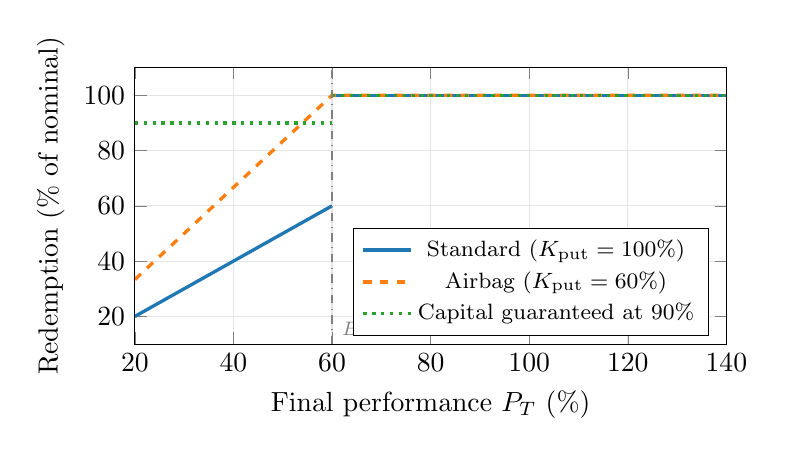
\begin{tikzpicture}
\begin{axis}[width=0.75\textwidth, height=0.42\textwidth, xmin=20, xmax=140, ymin=10, ymax=110,
             xlabel={Final performance $P_T$ (\%)}, ylabel={Redemption (\% of nominal)},
             grid=major, grid style={gray!20}, legend pos=south east, legend style={font=\footnotesize}]
\addplot[athena, very thick] coordinates {(20,20) (60,60)};
\addplot[athena, very thick, forget plot] coordinates {(60,100) (140,100)};
\addplot[nomemory, very thick, dashed] coordinates {(20,33.33) (60,100) (140,100)};
\addplot[american, very thick, dotted] coordinates {(20,90) (60,90)};
\addplot[american, very thick, dotted, forget plot] coordinates {(60,100) (140,100)};
\draw[gray, dashdotted] (axis cs:60,10) -- (axis cs:60,110) node[pos=0.06, right, font=\scriptsize] {$B^{\mathrm{prot}} = 60\%$};
\legend{Standard ($K_{\mathrm{put}} = 100\%$), Airbag ($K_{\mathrm{put}} = 60\%$), Capital guaranteed at 90\%}
\end{axis}
\end{tikzpicture}
\caption{Redemption at maturity of a note that was never called, European protection at 60\%.}
\label{fig:redemption}
\end{figure}

\subsection{Athena}
The Athena pays a coupon only with the redemption at the call date. If $\tau = t_k$, the investor receives
\begin{equation}
N(1 + c_k), \qquad c_k = \begin{cases} c\, t_k & \text{snowball (the coupons accumulate)}, \\ c\,(t_k - t_{k-1}) & \text{fixed coupon}, \end{cases}
\end{equation}
with $c$ the coupon rate per annum. If the note is not called, no coupon is paid and the redemption is
\eqref{eq:redemption}. A call at maturity ($P_T \ge B^{\mathrm{call}}_n$) pays the last coupon.

\subsection{Parametrisation}
Table~\ref{tab:parameters} lists the parameters of the class \code{Athena}; every variant of
Section~\ref{sec:athena} is one of these parameters changed.

\begin{table}[h]
\centering
\resizebox{\textwidth}{!}{%
\begin{tabular}{@{}lll@{}}
\toprule
\textbf{Feature} & \textbf{Parameter} & \textbf{Values} \\
\midrule
Maturity, initial fixing, nominal & \code{maturity}, \code{initial\_fixing}, \code{nominal} & years, index level, 100 \\
Observation dates & \code{frequency} or \code{observation\_dates} & monthly to annual, or any list ending at $T$ \\
Coupon rate & \code{coupon\_rate} & per annum, fraction of the nominal \\
Athena coupon & \code{coupon\_type} & \code{snowball}, \code{fixed} \\
Autocall barrier & \code{autocall\_barrier}, \code{step\_down} & fraction of $\Sref$, decrease per observation \\
Non-call period & \code{first\_call\_date} & years \\
Capital protection & \code{protection\_barrier}, \code{protection\_type} & fraction of $\Sref$; \code{european}, \code{american}, \code{american\_discrete} \\
Airbag, guarantee & \code{put\_strike}, \code{floor} & fraction of $\Sref$, fraction of the nominal \\
\bottomrule
\end{tabular}}
\caption{Parameters of the Athena (\code{Products/Athena/athena.py}).}
\label{tab:parameters}
\end{table}

\clearpage
% ==================================================================
\section{Market Data and Model}\label{sec:model}
% ==================================================================
The data are the CAC40 option chain of 12 February 2025 (spot $S_0 = 8042.19$, 142 quotes on 13 expiries from
9 days to 4.86 years) and the EURIBOR 6M zero-coupon curve. The forward curve $F(0,t)$ is bootstrapped from
put--call parity with a piecewise constant borrow-plus-dividend yield $q(t)$ \cite{benguedda2026heston}; its
integral reaches 0.136 at 4.86 years, so dividends lower the 4-year forward by about 11\% with respect to a zero
carry. Under $\Q$,
\begin{equation}
\frac{\dd S_t}{S_t} = \partial_t \ln F(0,t)\,\dd t + \sqrt{v_t}\,\dd W^S_t, \qquad
\dd v_t = \kappa(\theta - v_t)\,\dd t + \xi \sqrt{v_t}\,\dd W^v_t, \qquad \dd\langle W^S, W^v\rangle_t = \rho\,\dd t,
\end{equation}
with the parameters of Table~\ref{tab:heston}. The notes are struck at the money: $\Sref = S_0 = 8042.19$, and
$\Sref$ stays fixed when the Greeks bump the market. All the dates of the 4-year notes lie before the last listed
expiry (4.86 years).

\begin{table}[h]
\centering
\begin{tabular}{@{}cccccc@{}}
\toprule
$v_0$ & $\theta$ & $\kappa$ & $\xi$ & $\rho$ & IV RMSE \\
\midrule
0.0197 & 0.0438 & 1.308 & 0.482 & $-0.605$ & 0.421 vol pts \\
\bottomrule
\end{tabular}
\caption{Heston parameters calibrated on the CAC40 surface of 12 February 2025 \cite{benguedda2026heston}.}
\label{tab:heston}
\end{table}


\clearpage
% ==================================================================
\section{Pricing Method}\label{sec:method}
% ==================================================================

\subsection{Simulation}
The paths of $(S, v)$ are simulated with an Euler full truncation scheme on a weekly grid (52 steps a year,
208 steps for 4 years), the drift over each step being $\ln(F(0,t_{i+1})/F(0,t_i))$, so that
$\E[S_t] = F(0,t)$ at every date. $N = 50{,}000$ paths with antithetic variates are used (seed 42); prices and
standard errors are computed on the 25{,}000 independent pair averages. The observation dates are rounded to the
grid; with weekly steps, every monthly, quarterly, semi-annual and annual date falls within half a week of its
contractual date.

\subsection{Cash flows and protection}
For each path, the note is followed through its observation dates, each cash flow
being discounted with $D(0,t_k) = e^{-r(t_k) t_k}$. The knock-in indicator of \eqref{eq:redemption} is
\begin{itemize}
\item \emph{European}: $\ind_{\{P_T < B^{\mathrm{prot}}\}}$;
\item \emph{American continuous}: replaced by its conditional probability given the simulated path,
$1 - \prod_i (1 - p_i)$, where
$p_i = \exp\!\big(-2 \ln(S_{t_i}/H) \ln(S_{t_{i+1}}/H) / (v_{t_i}\Delta t)\big)$ is the probability that the
Brownian bridge of $\ln S$ touches $H = B^{\mathrm{prot}}\Sref$ between two grid dates \cite{beaglehole1997};
\item \emph{American daily}: the barrier is checked on a daily grid (252 steps a year).
\end{itemize}

\subsection{Variance reduction}
Besides antithetic variates, the discounted European put struck at $B^{\mathrm{prot}}\Sref$, whose Heston price
is known semi-analytically (Lewis formula), is used as a control variate with an optimal coefficient estimated on
the paths.

\subsection{Fair coupon and scenario statistics}
On a fixed set of paths, the call dates do not depend on the coupon, and every cash flow is affine in the coupon
rate $c$: the price is $V(c) = V(0) + c\,(V(1) - V(0))$, and the coupon that prices the note at par is
\begin{equation}
c^\star = \frac{N - V(0)}{V(1) - V(0)},
\end{equation}
obtained with two valuations. It excludes the issuer margin and funding spread. The same paths give the
probability of a call at each date, the probability to reach maturity, the probability of a capital loss
($\ind_{\mathrm{KI}} = 1$ and $P_T < K_{\mathrm{put}}$), the expected loss at maturity, the expected life
$\E[\min(\tau, T)]$ and the expected coupon paid.

\subsection{Greeks}
The Greeks are central finite differences with common random numbers \cite{glasserman2004}, on a nominal of 100:
Delta and Gamma (spot $\pm 1\%$, carry kept), Vega and Volga ($\sqrt{v_0}$ and $\sqrt{\theta}$ shifted by
$\pm 1$ vol point), Vanna, Rho ($\pm 10$bp on the zero curve, per $+1\%$), Dividend ($\pm 10$bp on $q(t)$, per
$+1\%$) and Theta (dates moved by one day). Delta is given per index point: multiply by $S_0/100 = 80.4$ for the
value change of a 1\% move. Each Greek is reported with its Monte Carlo standard error.

\subsection{Validation}
Three limit cases have a closed form (Table~\ref{tab:validation}). In a flat Black--Scholes
market ($S_0 = \Sref = 100$, $r = 3\%$, $q = 1\%$, $\sigma = 20\%$, $T = 2$, $N = 100$, Heston with $v_0 = \theta = \sigma^2$
and $\xi = 10^{-4}$, $10^5$ paths):
\begin{itemize}
\item a note never called (autocall barrier out of reach) with a European protection at $B = 60$ is worth
$N D(T) - \frac{N}{\Sref}\left[\mathrm{Put}(B) + (\Sref - B)\,\mathrm{DigitalPut}(B)\right]$;
\item with an American protection, $N D(T) - \frac{N}{\Sref}\,\mathrm{PDI}(K = \Sref, H = B)$ (Reiner--Rubinstein);
\item a note called for sure at $t_1$ is worth $N(1 + c\, t_1) D(t_1)$.
\end{itemize}

\begin{table}[h]
\centering
\resizebox{\textwidth}{!}{%
\begin{tabular}{@{}lrrrr@{}}
\toprule
\textbf{Case} & \textbf{Reference} & \textbf{Monte Carlo} & \textbf{Std error} & \textbf{Error / std error} \\
\midrule
Athena never called, European protection (flat) & 92.6369 & 92.6480 & 0.0141 & 0.79 \\
Athena never called, American protection (flat) & 91.5500 & 91.5483 & 0.0220 & $-0.07$ \\
Athena called for sure at $t_1 = 0.5$, $c = 8\%$ (flat) & 102.4516 & 102.4516 & 0 & exact \\
\bottomrule
\end{tabular}}
\caption{Validation of the pricer.}
\label{tab:validation}
\end{table}


\clearpage
% ==================================================================
\section{Athena : Base case}\label{sec:athena}
% ==================================================================


Let us consider, under the risk-neutral measure $\mathbb{Q}$, the general
case of an Athena in the base case. To lighten notation, we denote by
\begin{equation}
  E_i = \bigcap_{j=1}^{i-1} \{X_j < B_{ac}\}, \qquad i = 1, \dots, N,
  \qquad E_1 = \Omega,
\end{equation}
the event that the product has not been called before date $t_i$. The
event $\{\tau = t_i\}$ of an early redemption at date $t_i < T$ is then
$E_i \cap \{X_i \geq B_{ac}\}$, and $\{\tau = T\} = E_N$.

\subsection{Price of the Athena}

For a coupon $c$, the price of the Athena at inception is
\begin{equation}
  P_0 = \mathbb{E}^{\mathbb{Q}}\bigl[ D(\tau)\, \Pi_\tau \bigr],
\end{equation}
which, writing the autocall events explicitly, expands as
\begin{align}
  P_0 = {}& \sum_{i=1}^{N-1} D(t_i)\,(1 + i c)\,
          \mathbb{Q}\bigl( E_i \cap \{X_i \geq B_{ac}\} \bigr) \nonumber \\
        & + D(T)\,(1 + N c)\,
          \mathbb{Q}\bigl( E_N \cap \{X_N \geq B_{ac}\} \bigr) \nonumber \\
        & + D(T)\,
          \mathbb{Q}\bigl( E_N \cap \{B_p \leq X_N < B_{ac}\} \bigr) \nonumber \\
        & + D(T)\,
          \mathbb{E}^{\mathbb{Q}}\bigl[ X_N \, \ind_{E_N \cap \{X_N < B_p\}} \bigr].
  \label{eq:athena-price-explicit}
\end{align}
The first term corresponds to an early redemption at date $t_i$, the
second to a redemption with coupons at maturity, the third to the
repayment of the notional only, and the last one to the capital loss
scenario.

\subsection{Linearity in the coupon and embedded put}

We now turn to the determination of the fair coupon level $c$. A basic
Athena has the convenient property that its price is affine in the
coupon. Indeed, the coupon only affects the \emph{amount} paid at
redemption, never the redemption time $\tau$, which depends on the path
of the underlying alone. Moreover, on the event $E_N$ that the product has
not been called before maturity, the terminal payoff can be rewritten,
since $B_p < 1$, as
\begin{equation}
  \Pi_T = 1 + N c\, \ind_{\{X_N \geq B_{ac}\}}
        - (1 - X_N)^+ \, \ind_{\{X_N < B_p\}} .
  \label{eq:athena-terminal-payoff}
\end{equation}
The last term is the payoff of a down-and-in put with strike $100\%$ and
barrier $B_p$ observed at maturity, which is sold by the investor.
Substituting \eqref{eq:athena-terminal-payoff} into
\eqref{eq:athena-price-explicit} yields the decomposition
\begin{equation}
  P_0 = \underbrace{\mathbb{E}^{\mathbb{Q}}\bigl[ D(\tau) \bigr]}_{\text{notional}}
      + c \underbrace{\sum_{i=1}^{N} i\, D(t_i)\,
        \mathbb{Q}\bigl( E_i \cap \{X_i \geq B_{ac}\} \bigr)}_{B \ (\text{coupons})}
      - \underbrace{D(T)\, \mathbb{E}^{\mathbb{Q}}\Bigl[ (1 - X_N)^+ \,
        \ind_{\{X_N < B_p\}}\, \ind_{E_N} \Bigr]}_{\mathrm{PDI}^{ac}} .
  \label{eq:athena-pdi}
\end{equation}
The investor is thus long a note repaying the notional at the random time
$\tau$, long a strip of conditional coupons, and short a down-and-in put
$\mathrm{PDI}^{ac}$. Grouping the terms that do not depend on the coupon,
the price takes the affine form
\begin{equation}
  P_0 = A + c\, B,
  \qquad
  A = \mathbb{E}^{\mathbb{Q}}\bigl[ D(\tau) \bigr] - \mathrm{PDI}^{ac},
\end{equation}
where $A$ is the price of the same product with a zero coupon, and $B$
the value of a unit coupon paid in all scenarios where coupons are
received.

\subsection{Fair coupon}

The fair coupon $c^\star$ is the coupon for which the price equals a
target $P^\star$, namely $P^\star = 1$ for a fair price, or
$P^\star = 1 - m$ when the issuer retains a margin $m$. By linearity, it
is given in closed form by
\begin{equation}
  \boxed{\,c^\star = \frac{P^\star - A}{B}
  = \frac{P^\star - \mathbb{E}^{\mathbb{Q}}\bigl[ D(\tau) \bigr] + \mathrm{PDI}^{ac}}{B}\,}
  \label{eq:fair-coupon}
\end{equation}
To determine the root of this equation, a single Monte Carlo
simulation provides $A$ and $B$, hence $c^\star$. This expression also
makes the economics of the product transparent: the coupons finance the
down-and-in put sold by the investor, together with the funding benefit
of the issuer, since $\mathbb{E}^{\mathbb{Q}}[D(\tau)] < 1$ as soon as
cash flows are discounted with a positive rate and funding spread.

\subsection{Remarks on the embedded put}

The put $\mathrm{PDI}^{ac}$ is not a vanilla barrier option: it is
knocked out whenever the product is autocalled, which is captured by the
indicator $\ind_{E_N}$. Since $\ind_{E_N} \leq 1$, its value is bounded by
that of the standard European down-and-in put,
\begin{equation}
  \mathrm{PDI}^{ac} \leq \mathrm{PDI}
  = D(T)\, \mathbb{E}^{\mathbb{Q}}\Bigl[ (1 - X_N)^+ \, \ind_{\{X_N < B_p\}} \Bigr].
\end{equation}
The latter itself decomposes into a vanilla put struck at the barrier
and a digital put,
\begin{equation}
  (1 - X_N)^+ \, \ind_{\{X_N < B_p\}}
  = (B_p - X_N)^+ + (1 - B_p)\, \ind_{\{X_N < B_p\}},
\end{equation}
so that, absent the autocall feature, its value follows directly from the
implied volatility surface around strike $B_p$, the digital term making
it sensitive to the skew.



\subsection{Structuration :}

From the investor's perspective, the basic Athena note is composed of:
\begin{itemize}
  \item a long position in an \emph{autocallable zero-coupon note} with
        maximal maturity $T$, which repays the notional together with the
        accrued coupons at the first observation date $t_i$ such that
        $X_i \geq B_{ac}$, and the notional alone at maturity otherwise;
  \item a short position in a \emph{down-and-in put} (PDI) with strike
        $100\%$ and barrier $B_p$ observed at maturity, which is knocked
        out whenever the product is autocalled.
\end{itemize}


\subsection{Sensitivity analysis :}

We will now look at the different sensitivities of the product and what are the impacts of a move on certain parameters on $c$. We are now thinking from the investor point of view and with an already contracted note.


\subsection*{Volatility}

The investor is short PDI then he is short $\nu$. The PDI price decreases with volatility so an increase of the volatility will decrease the value of the note.

If the product is not contracted yet it will incread the proba to call the product and then it increases the coupon paid to the investor.


\subsection*{Protection barrier}

If the protection barrier is higher, then it is more probable to cross it and it reduces the price of the note. The effect on the coupon $c$ is that it is increased.


\subsection*{Recall Barrier}


If the recall barrier is increased, it is less probable to be recall before maturity, then it increases the coupon $c$.


\subsection*{Dividend}


If the underlying asset increases its dividend, it increases the value of $c$


Peut etre parce que l'investisseur ne touche pas les dividendes donc demandera une rémunération plus élevée.


\subsection*{Spread}




\subsection*{Risk free rate}




\subsection*{Maturity}




\subsection*{Skew}






\subsection*{Correlation}





\subsection{Pricing : A numerical example}


Let us now consider a synthetic Athena issued by a risky issuer, which
requires taking into account the credit spread of the issuer. The product
is written on the CAC~40 index (dividends not reinvested). Its initial level
is fixed on 31 January 2025 and it matures in November 2027. A coupon $c$
accrues every quarter and is paid upon redemption. The underlying is
observed quarterly: at each observation date, the product is redeemed
early if the index closes at or above $100\%$ of its initial level. If
the product has not been called, the investor receives at maturity the
notional plus the accrued coupons if the index is at or above its initial
level, the notional alone if it is at or above the protection barrier
$B_p = 60\%$, and the notional reduced by the full decline of the index
otherwise.

\subsubsection{Model}

\subsubsection{Pricing}

\subsubsection{Sensitivities}

\subsection{Features of Athena products}

\subsubsection{Exercise frequency}

\subsubsection{Step-down barrier}

\subsubsection{Airbag}

\subsubsection{Buffer}

\subsubsection{Guaranteed capital}

\subsubsection{Coupon range accrual}

\subsubsection{Duo mechanism}

\subsubsection{Look back}

























\begin{figure}[h]
\centering
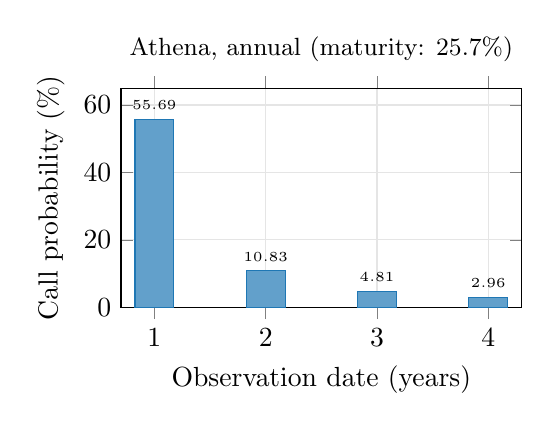
\begin{tikzpicture}
\begin{axis}[width=0.55\textwidth, height=0.36\textwidth, ymin=0, ymax=65, ylabel={Call probability (\%)},
  grid=major, grid style={gray!20}, title style={font=\small}, ybar, bar width=14pt,
  xlabel={Observation date (years)}, xtick={1,2,3,4}, title={Athena, annual (maturity: 25.7\%)},
  nodes near coords, every node near coord/.append style={font=\tiny}]
\addplot[fill=athena!70, draw=athena] coordinates {(1,55.69) (2,10.83) (3,4.81) (4,2.96)};
\end{axis}
\end{tikzpicture}
\caption{Base Athena: probability of being called at each observation date (autocall barrier at 100\%).}
\label{fig:call_probabilities}
\end{figure}

\begin{figure}[h]
\centering
\figfile{athena_scenarios.png}{0.9\textwidth}
\caption{Base Athena: simulated paths of the performance, grouped by outcome.}
\label{fig:athena_scenarios}
\end{figure}

\subsection{All the forms of the Athena}
Table~\ref{tab:athena_variants} changes one feature of the base case at a time. All prices are computed at
the same coupon of 8\% (standard errors between 0.03 and 0.08); the fair coupon is the comparable quantity.

\begin{table}[h]
\centering
\resizebox{\textwidth}{!}{%
\begin{tabular}{@{}lrrrrrrr@{}}
\toprule
\textbf{Variant} & \textbf{Price at 8\%} & \textbf{Fair coupon} & \textbf{P(call $t_1$)} & \textbf{P(maturity)} & \textbf{P(loss)} & \textbf{E[loss]} & \textbf{E[life]} \\
 & & \textbf{(\% p.a.)} & \textbf{(\%)} & \textbf{(\%)} & \textbf{(\%)} & \textbf{(\%)} & \textbf{(y)} \\
\midrule
Base (annual, snowball, AC 100\%, EU 60\%) & 98.60 & 9.41 & 55.69 & 25.70 & 9.06 & 5.27 & 2.06 \\
Semi-annual observations & 98.64 & 9.93 & 53.30 & 18.61 & 6.97 & 4.08 & 1.48 \\
Quarterly observations & 98.77 & 10.54 & 55.43 & 13.29 & 5.22 & 3.05 & 1.03 \\
Monthly observations & 99.16 & 11.11 & 56.21 & 7.77 & 3.13 & 1.83 & 0.59 \\
Fixed coupon (no snowball) & 96.40 & 13.00 & 55.69 & 25.70 & 9.06 & 5.27 & 2.06 \\
Autocall barrier 90\% & 100.95 & 7.03 & 77.37 & 13.24 & 6.41 & 3.77 & 1.54 \\
Autocall barrier 110\% & 95.40 & 12.71 & 25.07 & 45.60 & 11.77 & 6.77 & 2.85 \\
Step-down 5\% per year & 100.65 & 7.46 & 55.69 & 17.56 & 8.57 & 5.01 & 1.95 \\
Quarterly, non-call 1 year & 99.09 & 8.94 & 0.00 & 22.06 & 8.42 & 4.92 & 1.89 \\
Protection 50\% & 99.90 & 8.10 & 55.69 & 25.70 & 5.91 & 3.86 & 2.06 \\
Protection 70\% & 97.33 & 10.68 & 55.69 & 25.70 & 12.96 & 6.63 & 2.06 \\
American protection (continuous) & 96.83 & 11.18 & 55.69 & 25.70 & 16.43 & 7.20 & 2.06 \\
American protection (daily) & 96.95 & 11.05 & 55.53 & 25.67 & 16.07 & 7.18 & 2.07 \\
Airbag & 100.89 & 7.10 & 55.69 & 25.70 & 9.06 & 2.75 & 2.06 \\
Capital guaranteed 90\% & 102.56 & 5.42 & 55.69 & 25.70 & 9.06 & 0.91 & 2.06 \\
Capital guaranteed 100\% & 103.39 & 4.59 & 55.69 & 25.70 & 0.00 & 0.00 & 2.06 \\
Buffer\\
\bottomrule
\end{tabular}}
\caption{Athena variants on the CAC40 (Heston, 50{,}000 paths). E[loss] in \% of the nominal.}
\label{tab:athena_variants}
\end{table}

\paragraph{Reading the table.} The investor is short a down-and-in put whose premium is paid back through the
coupons; the fair coupon per annum is roughly this premium divided by the expected life of the note.
\begin{itemize}
\item \emph{Observation frequency.} More frequent observations call the note earlier (expected life from 2.06 to
0.59 years) and reduce the probability of a loss (from 9.06\% to 3.13\%), but the put premium is spread over a much
shorter life: the fair coupon rises from 9.41\% to 11.11\%.
\item \emph{Snowball vs fixed coupon.} A fixed coupon pays $c$ once whatever the call date, instead of $c\,t_k$:
the fair coupon is 13.00\% instead of 9.41\%.
\item \emph{Autocall barrier.} A barrier at 90\% calls 77\% of the notes after one year and lowers the fair coupon
to 7.03\%; at 110\%, 46\% of the notes reach maturity and the fair coupon is 12.71\%. A step-down of 5\% a year
lowers it to 7.46\%.
\item \emph{Protection.} Each 5 points of protection barrier move the fair coupon by 0.4 to 0.7 point
(Figure~\ref{fig:fair_coupon}). The American protection raises the probability of a loss from 9.06\% to 16.43\% and
the fair coupon by 1.77 points; a daily monitoring lowers the fair coupon by 0.13 point with respect to a continuous
monitoring.
\item \emph{Airbag and guarantee.} The airbag halves the expected loss (2.75\% instead of 5.27\%) for a coupon of
7.10\%; a 100\% capital guarantee leaves a coupon of 4.59\%, the value of the call-at-par feature on top of a
zero-coupon bond.
\end{itemize}

\begin{figure}[h]
\centering
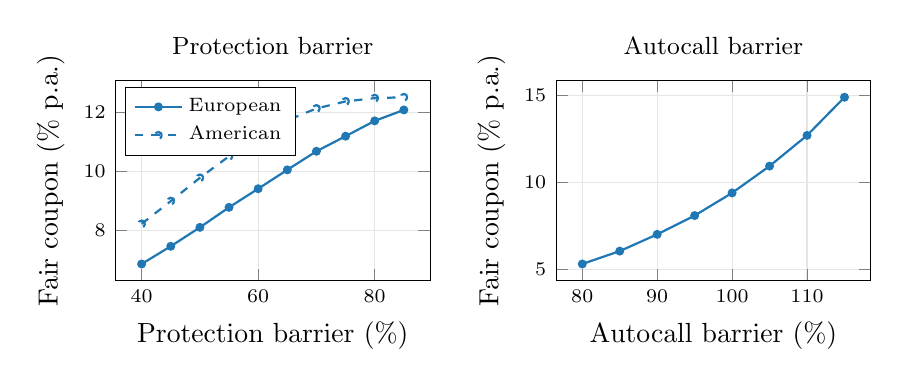
\begin{tikzpicture}
\begin{groupplot}[group style={group size=2 by 1, horizontal sep=1.6cm},
  width=0.46\textwidth, height=0.34\textwidth, ylabel={Fair coupon (\% p.a.)}, grid=major, grid style={gray!20},
  title style={font=\small}, legend style={font=\scriptsize, at={(0.03,0.97)}, anchor=north west}, ticklabel style={font=\scriptsize}]
\nextgroupplot[xlabel={Protection barrier (\%)}, title={Protection barrier}]
\addplot[athena, thick, mark=*, mark size=1.2pt] coordinates {(40,6.86) (45,7.46) (50,8.10) (55,8.78) (60,9.41) (65,10.05) (70,10.68) (75,11.19) (80,11.71) (85,12.08)};
\addplot[athena, thick, dashed, mark=o, mark size=1.2pt] coordinates {(40,8.22) (45,8.99) (50,9.78) (55,10.51) (60,11.18) (65,11.73) (70,12.13) (75,12.37) (80,12.48) (85,12.51)};
\legend{European, American}
\nextgroupplot[xlabel={Autocall barrier (\%)}, title={Autocall barrier}]
\addplot[athena, thick, mark=*, mark size=1.2pt] coordinates {(80,5.33) (85,6.07) (90,7.03) (95,8.11) (100,9.41) (105,10.95) (110,12.71) (115,14.90)};
\end{groupplot}
\end{tikzpicture}
\caption{Athena: fair coupon as a function of the barriers (other features of the base case unchanged; American:
continuous monitoring).}
\label{fig:fair_coupon}
\end{figure}

\subsection{Greeks}
Table~\ref{tab:athena_greeks} gives the Greeks of five Athena variants. Gamma and Volga are not significant at
this number of paths (base case: Gamma $-3.0 \times 10^{-6} \pm 5.4 \times 10^{-6}$, Volga $-0.042 \pm 0.037$);
the other Greeks have relative standard errors between 3\% and 45\% (base case: Delta $0.00506 \pm 0.00019$, Vega
$-0.549 \pm 0.016$, Rho $-0.77 \pm 0.07$, Dividend $-1.12 \pm 0.07$, Theta $0.0050 \pm 0.0016$).

\begin{table}[h]
\centering
\resizebox{\textwidth}{!}{%
\begin{tabular}{@{}lrrrrrrrr@{}}
\toprule
\textbf{Athena} & \textbf{Price} & \textbf{Delta} & \textbf{Delta 1\%} & \textbf{Vega} & \textbf{Vanna} & \textbf{Rho} & \textbf{Dividend} & \textbf{Theta} \\
 & & (per point) & (per 1\% move) & (per vol pt) & ($\times 10^{4}$) & (per 1\%) & (per 1\%) & (per day) \\
\midrule
Base & 98.60 & 0.00506 & 0.407 & $-0.549$ & 2.51 & $-0.770$ & $-1.115$ & 0.0050 \\
American protection & 96.83 & 0.00644 & 0.518 & $-0.657$ & 1.97 & $-0.546$ & $-1.269$ & 0.0050 \\
Step-down 5\% & 100.65 & 0.00321 & 0.258 & $-0.637$ & 6.36 & $-0.900$ & $-0.935$ & 0.0079 \\
Airbag & 100.89 & 0.00343 & 0.276 & $-0.354$ & 1.28 & $-1.161$ & $-0.815$ & 0.0037 \\
Guaranteed 90\% & 102.56 & 0.00241 & 0.193 & $-0.139$ & 0.44 & $-1.436$ & $-0.608$ & 0.0023 \\
\bottomrule
\end{tabular}}
\caption{Greeks of Athena variants (nominal 100, coupon 8\%).}
\label{tab:athena_greeks}
\end{table}

The note is long the index (a 1\% rise is worth 0.41 on 100) and short volatility: one vol point costs 0.55, the
short put dominating the long digital-like call features. It is also short dividends: one point of carry lowers
every forward and costs 1.12, twice the vega. It loses with higher rates (discounting of the coupons and of the
nominal) and earns about 0.005 a day (1.8 a year) as the put decays. The capital guarantee reduces every risk but
the rate risk, since the guaranteed redemption behaves as a zero-coupon bond. Figure~\ref{fig:athena_greeks}
displays the table with 95\% confidence intervals and Figure~\ref{fig:athena_profiles} the Greeks as functions of
the spot, the initial fixing staying at 8042: the Delta increases as the spot falls towards the protection barrier
(4825), and peaks just above it with an American protection.

\begin{figure}[h]
\centering
\figfile{athena_greeks.png}{\textwidth}
\caption{Greeks of the Athena variants with 95\% confidence intervals.}
\label{fig:athena_greeks}
\end{figure}

\begin{figure}[h]
\centering
\figfile{athena_profiles.png}{\textwidth}
\caption{Athena: price and Greeks as functions of the spot (30{,}000 paths, spot step 400).}
\label{fig:athena_profiles}
\end{figure}

\paragraph{Sensitivities to the Heston parameters.} Per unit of parameter, the base Athena has
$\partial V/\partial v_0 = -69.9$, $\partial V/\partial \theta = -69.4$, $\partial V/\partial \kappa = -0.81$,
$\partial V/\partial \xi = 3.94$ and $\partial V/\partial \rho = -1.03$. The note loses with the variance level
(short put) and gains with the vol-of-vol $\xi$.

% ==================================================================
\section{Implementation}\label{sec:implementation}
% ==================================================================

\subsection{Code}
\begin{itemize}
\item \code{Products/Athena/athena.py}: the self-contained class \code{Athena} (contract, \code{path\_payoff},
\code{fair\_coupon}, \code{statistics});
\item \code{Equity\_Models/monte\_carlo.py}: \code{MonteCarloPricer}, which simulates the paths and calls
\code{path\_payoff} for products with several cash flows;
\item \code{Equity\_Models/Heston.py}, \code{Equity\_Models/forward\_curve.py}: calibrated model and forward curve;
\item \code{Equity\_Models/greeks.py}: Greeks with common random numbers, including the Dividend Greek;
\item \code{Products/market.py}: CAC40 market data and calibrated Heston model (\code{cac40\_heston});
\item \code{Products/notes\_analysis.py}: comparison of variants and plots;
\item notebooks \code{Products/Athena/athena\_pricer.ipynb} and\\
\code{Products/Athena/athena\_synthetic\_pricing.ipynb}.
\end{itemize}

\begin{lstlisting}
from market import cac40_heston
from athena import Athena
from Equity_Models.monte_carlo import MonteCarloPricer
from Equity_Models.greeks import Greeks

mkt = cac40_heston()
pricer = MonteCarloPricer(n_paths=50_000, steps_per_year=52, seed=42)
note = Athena(4.0, mkt.S0, 0.08, coupon_type="snowball", frequency=1.0,
              autocall_barrier=1.0, protection_barrier=0.6, protection_type="european")
print(pricer.price(mkt.heston, note))              # price and standard error
print(note.fair_coupon(pricer, mkt.heston))        # coupon p.a. at par
print(note.statistics(pricer, mkt.heston))         # call probabilities, loss, life, coupon
print(Greeks(pricer).compute(mkt.heston, note, Greeks.ORDER))
\end{lstlisting}

\subsection{Cost}
With $N$ paths and $M$ steps, the simulation costs $\mathcal{O}(NM)$ in time and stores $S$ and $v$, i.e.
$16(M+1)N$ bytes: 167 MB for $N = 50{,}000$ and the weekly grid of 4 years, 807 MB on a daily grid. Following the
note through its $n$ observation dates costs $\mathcal{O}(nN)$, the American continuous protection
$\mathcal{O}(NM)$. Measured times (one CPU core): 0.30 s for a valuation including the simulation; 0.02 to 0.12 s
for the price, the fair coupon and the statistics of a variant on cached paths (1.5 s with an American
protection); 26 s for the eight Greeks of five notes (14 valuations each); 41 to 44 s for the spot profiles of
four notes (16 spots $\times$ 6 scenarios, 30{,}000 paths).

% ==================================================================
\section{Limitations and Next Steps}\label{sec:limitations}
% ==================================================================
\begin{itemize}
\item \emph{Single underlying.} Most autocalls sold today are worst-of on two to four indices or stocks; they need
a multi-asset model and a correlation calibration.
\item \emph{Model.} The value of an autocall depends on the forward skew and on the joint dynamics of spot and
volatility between observation dates; a pure Heston model with constant parameters is not the market standard,
which is a local stochastic volatility model calibrated to the whole surface \cite{bergomi2016}.
\item \emph{Fair coupon.} It prices the note at par without issuer margin, funding spread or issuer credit risk; a
real issue price is below par by the margin.
\item \emph{Discretisation.} Euler full truncation with the Feller condition violated ($2\kappa\theta/\xi^2 = 0.49$),
weekly grid with the variance frozen over each week for the Brownian bridge.
\item \emph{Greeks.} Gamma and Volga are not significant with 50{,}000 paths: the payoff jumps at the autocall and
protection barriers.
\item \emph{Dividends.} Continuous dividend yield bootstrapped from the forwards; real notes are exposed to
discrete dividends and to dividend risk, which the Dividend Greek only measures for a parallel shift.
\end{itemize}

% ==================================================================
\section{Conclusion}
% ==================================================================
A single parametrisation covers the Athena with all its usual features, and a Monte Carlo pricer under a
calibrated Heston model recovers three exact limit cases within one standard error. On the CAC40 of
12 February 2025, the base 4-year Athena pays 9.41\% a year; the protection type is the most expensive feature for
the investor (1.77 point of coupon for an American protection); more frequent observations raise the fair coupon,
and a step-down of the autocall barrier lowers it. The note is short volatility and short dividends, the dividend
exposure being twice the vega.

% ==================================================================
\appendix
\section{Notation}
% ==================================================================
\begin{center}
\begin{tabular}{@{}ll@{}}
\toprule
Symbol & Meaning \\
\midrule
$N$, $\Sref$, $T$ & Nominal, initial fixing, maturity \\
$t_k$, $\delta_k = t_k - t_{k-1}$ & Observation dates and accrual periods \\
$P_k = S_{t_k}/\Sref$ & Performance at $t_k$ \\
$B^{\mathrm{call}}_k$, $B^{\mathrm{prot}}$ & Autocall and protection barriers (fractions of $\Sref$) \\
$c$, $c^\star$ & Coupon rate per annum, fair coupon \\
$K_{\mathrm{put}}$, $\phi$ & Strike of the short put, capital floor \\
$\tau$ & Call date \\
$\ind_{\mathrm{KI}}$ & Knock-in event of the protection \\
\bottomrule
\end{tabular}
\end{center}

% ==================================================================
\begin{thebibliography}{99}
\bibitem{benguedda2026heston} E. Benguedda, \emph{Calibration of the Heston Stochastic Volatility Model: Theoretical
Framework, Numerical Methods, and Limitations}, 2026.
\bibitem{benguedda2026phoenix} E. Benguedda, \emph{Phoenix Autocallable Notes on the CAC40 under a Calibrated Heston
Model: Fair Coupons, Scenarios and Greeks}, 2026.
\bibitem{benguedda2026barrier} E. Benguedda, \emph{Monte Carlo Pricing and Greeks of Single Barrier Options under a
Calibrated Heston Model}, 2026.
\bibitem{heston1993} S. L. Heston, A closed-form solution for options with stochastic volatility with applications
to bond and currency options, \emph{Review of Financial Studies}, 6(2):327--343, 1993.
\bibitem{bouzoubaa2010} M. Bouzoubaa and A. Osseiran, \emph{Exotic Options and Hybrids: A Guide to Structuring,
Pricing and Trading}, Wiley, 2010.
\bibitem{bergomi2016} L. Bergomi, \emph{Stochastic Volatility Modeling}, Chapman and Hall/CRC, 2016.
\bibitem{glasserman2004} P. Glasserman, \emph{Monte Carlo Methods in Financial Engineering}, Springer, 2004.
\bibitem{beaglehole1997} D. R. Beaglehole, P. H. Dybvig and G. Zhou, Going to extremes: correcting simulation bias
in exotic option valuation, \emph{Financial Analysts Journal}, 53(1):62--68, 1997.
\bibitem{reiner1991} E. Reiner and M. Rubinstein, Breaking down the barriers, \emph{Risk}, 4(8):28--35, 1991.
\bibitem{andersen2008} L. Andersen, Simple and efficient simulation of the Heston stochastic volatility model,
\emph{Journal of Computational Finance}, 11(3):1--42, 2008.
\end{thebibliography}

\end{document}
